\chapter{Introduction}

%Replace \lipsum with text.
% You may have as many sections as you please. This is just for reference.

\section{Objective}

Our objective is to create library with some set of functionalities to detect anomalies in the give input time series​. Anomalies will be based on the hypothesis stated by the user​. For particular scenario stated by user, execute appropriate algorithms and report the anomalies in the time series.

%You should cite papers in the following manner: Bayliss et al.~\cite{Bay1} gave an iterative method for Helmholtz equation etc.
%Similar work has been done in \cite{Bailey,Ernst,Gold3}.


\section{Motivation}

Supply demand imbalance, natural calamities etc. may not always be the reason behind the rise in the price of a commodity. ​It may be a consequence of artificial supply deficit planned intelligently by traders’ nexus for profiteering through manipulation of supply of commodity and hence indirectly controlling their prices. ​Our attempt is to locate such hikes in prices which seem suspicious (we call them anomalies).​ To detect and analyse the characteristics of anomalies in the prices of commodities. Currently we have considered the case of onion and based on that we are looking forward to develop library for any time-series.

\section{Related Work}

Supply demand imbalance, natural calamities etc. may not always be the reason behind the rise in the price of a commodity. ​It may be a consequence of artificial supply deficit planned intelligently by traders’ nexus for profiteering through manipulation of supply of commodity and hence indirectly controlling their prices. ​Our attempt is to locate such hikes in prices which seem suspicious (we call them anomalies).​ To detect and analyse the characteristics of anomalies in the prices of commodities. Currently we have considered the case of onion and based on that we are looking forward to develop library for any time-series.


% You may add figures in the following manner.
\begin{figure}[here]
\begin{center}	
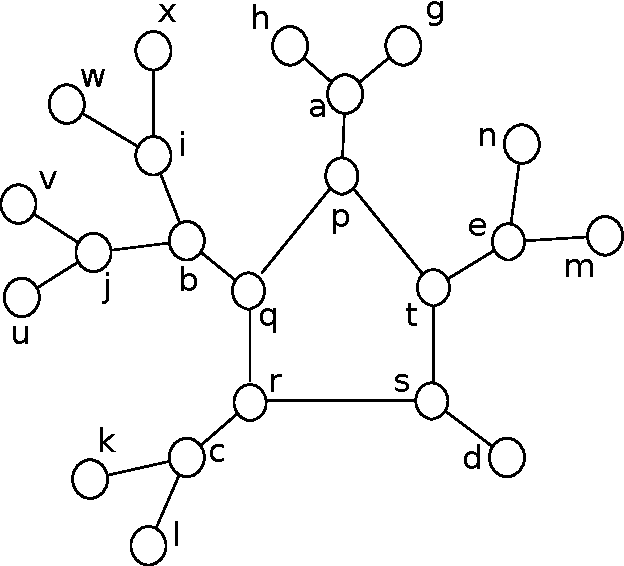
\includegraphics[scale=0.4]{pent} 
\caption{Pentagon $pqrst$}
\label{fig:pent}
\end{center}
\end{figure}

\lipsum[1]

\section{SECTION NAME}
\lipsum[2]

\begin{table}
\centering
\begin{tabular}{| c | c |}
\hline
{\bf item 1} & {\bf item 2} \\ \hline
%
abcde & 5 \\ \hline
%
pqrst & 4 \\ \hline
\end{tabular}
\caption{A sample table}
\label{table:1}
\end{table}
